\documentclass{article}
\usepackage{graphicx}
\usepackage{float}
\usepackage[utf8]{vietnam}
\usepackage{lipsum}
\usepackage{tikz}
\usepackage{tikzpagenodes}
\usetikzlibrary{calc}
\usepackage[a4paper, top=2cm, bottom=2cm, left=3.5cm, right=2.5cm]{geometry}
\usepackage{pdfpages}
\usepackage{hyperref}
\usepackage{amsmath}
\usepackage{enumitem} % Gói hỗ trợ tùy chỉnh danh sách
\usepackage{xcolor}
\usepackage{tcolorbox} % Gói hỗ trợ tùy chỉnh khung
\usepackage{makecell} % Gói hỗ trợ tạo ô trong bảng
% \usetikzlibrary{arrows.meta}
% \usepackage{rotating} % Bắt buộc phải có
% \usepackage{pdflscape} % Khuyên dùng pdflscape thay vì lscape để PDF xoay đúng chiều khi xem trên máy tính

\setlength{\parindent}{0pt} % Không thụt lề

\definecolor{RedHUST}{RGB}{205,5,5}
% \setlist{format={\color{RedHUST}\bfseries}} % Đặt màu cho danh sách


% Định nghĩa lại lệnh \lipsum gốc để tự động bọc trong màu RedHUST
\let\oldlipsum\lipsum
\renewcommand{\lipsum}[1][1-7]{{\color{RedHUST}\oldlipsum[#1]}}


\definecolor{BlueSAMI}{RGB}{1,90,143}
\setlist{format={\color{BlueSAMI}\bfseries}} % Đặt màu cho danh sách

% Định nghĩa môi trường block
\newenvironment{block}[1]
{\begin{tcolorbox}[%
colback=white, % Màu nền nội dung
colframe=BlueSAMI, % Màu khung
arc=3mm, % Góc bo tròn
title={\textbf{#1}}, % Tiêu đề, in đậm
colbacktitle=BlueSAMI, % Màu nền tiêu đề
coltitle=white, % Màu chữ tiêu đề
boxrule=2pt, % Độ dày của khung
before upper={\tcbtitle\vskip0pt\par}
]
\begin{minipage}{\textwidth}}
{\end{minipage}
\end{tcolorbox}}

\setlength{\headheight}{12.42429pt} % bug header foooter
\usepackage{fancyhdr}
\pagestyle{fancy}
\lhead{Đồ án tốt nghiệp}
\rhead{Vũ Văn Nghĩa - 20206205}
\renewcommand{\headrulewidth}{0.4pt}
\renewcommand{\footrulewidth}{0.4pt}

% Căn giữa tiêu đề mục lục
\makeatletter
\renewcommand{\tableofcontents}{
\begin{center}
\section*{\contentsname}
\end{center}
\@starttoc{toc}
}
\makeatother

\numberwithin{figure}{section} % Đặt số ảnh theo section
% Căn giữa tiêu đề danh sách hình ảnh
\makeatletter
\renewcommand{\listoffigures}{
\begin{center}
\section*{\listfigurename}
\end{center}
\@starttoc{lof}
}
\makeatother

% \usepackage{microtype}
% \usepackage{blindtext}

\usepackage{titlesec}
\newcommand{\sectionbreak}{\clearpage}

\begin{document}

% \input{contents/0/trang_bia/trang_bia}
% \input{contents/0/trang_bia/trang_bia}
% \input{contents/0/trang_trang/trang_trang}

% % 
\includepdf[pages=-]{contents/0/bao_cao/nhan_xet.pdf}
% % 
\includepdf[pages=-]{contents/0/bao_cao/bao_cao_1.pdf}
% % 
\includepdf[pages=-]{contents/0/bao_cao/bao_cao_2.pdf}
% % 
\includepdf[pages=-]{contents/0/bao_cao/danh_gia.pdf}

% \input{contents/0/loi_cam_on_tom_tat/loi_cam_on_tom_tat}
\input{contents/0/muc_luc/muc_luc}

\input{contents/0/danh_muc/DANH_MUC_KY_HIEU}
\input{contents/0/danh_muc/DANH_MUC_HINH_VE}
% DANH MỤC BẢNG BIỂU

\newpage

\renewcommand{\listtablename}{DANH MỤC BẢNG BIỂU}
\makeatletter
\renewcommand{\listoftables}{
\begin{center}
\section*{\listtablename}
\end{center}
\@starttoc{lot}
}
\makeatother
\addcontentsline{toc}{section}{DANH MỤC BẢNG BIỂU}
{\let\oldnumberline\numberline
\renewcommand{\numberline}{Bảng~\oldnumberline}
\listoftables}

\newpage


\input{contents/Tong_quan_ve_he_thong} % Tổng quan về hệ thống
\subsection{Mục tiêu và Phạm vi dự án}

\subsubsection{Mục tiêu tổng quan}
Mục tiêu tổng quan của dự án là nghiên cứu và xây dựng một hệ thống trợ lý pháp luật thông minh ứng dụng công nghệ Trí tuệ nhân tạo (AI) và Kiến trúc vi dịch vụ (Microservices). Hệ thống nhằm hỗ trợ người dùng và các chuyên gia pháp lý tra cứu, giải đáp các câu hỏi về hệ thống văn bản pháp luật Việt Nam một cách nhanh chóng, chính xác, với các bước lập luận rõ ràng và trích dẫn nguồn văn bản pháp lý chính thống.

\subsubsection{Mục tiêu cụ thể}

Để đạt được mục tiêu tổng quan, dự án hướng tới hoàn thành các mục tiêu cụ thể về mặt tính năng và trải nghiệm người dùng như sau:

\begin{itemize}
\item \textbf{Đảm bảo an toàn thông tin và định danh chuẩn xác}: Xây dựng cơ chế quản lý tài khoản linh hoạt, tích hợp các phương thức xác thực đa yếu tố nhằm bảo vệ tối đa dữ liệu và quyền riêng tư của người dùng.

\item \textbf{Nâng cao tính minh bạch và độ tin cậy trong tư vấn pháp lý}: Xử lý các truy vấn pháp lý phức tạp bằng cách không chỉ đưa ra câu trả lời cuối cùng, mà còn phải diễn giải chi tiết quá trình suy luận và cung cấp chính xác các nguồn tài liệu tham khảo.

\item \textbf{Tối ưu hóa khả năng tiếp cận và tương tác đa giác quan}: Xóa bỏ rào cản nhập liệu truyền thống bằng cách cung cấp trải nghiệm đàm thoại rảnh tay, cho phép người dùng tương tác trực tiếp với hệ thống qua giọng nói tự nhiên.

\item \textbf{Xây dựng mô hình cung cấp dịch vụ bền vững}: Thiết lập hệ thống phân quyền linh hoạt giữa các nhóm người dùng, đi kèm với quy trình thanh toán tự động, liền mạch để quản lý các gói dịch vụ cao cấp.
\end{itemize}

\subsubsection{Phạm vi dự án}
Dự án tập trung nghiên cứu, thiết kế và phát triển các thành phần cốt lõi trong một hệ thống vi dịch vụ, giới hạn trong các phạm vi sau:

\begin{itemize}
\item \textbf{Phân hệ Quản trị người dùng \& Bảo mật}: Cài đặt hệ thống xác thực thông qua Supabase Auth, hỗ trợ đăng nhập Email/Mật khẩu, Google OAuth và xác thực hai yếu tố (2FA - TOTP).

\item \textbf{Phân hệ Thu thập dữ liệu pháp luật}: Thiết lập đường ống (Data Pipeline) tự động thu thập và đồng bộ hóa văn bản quy phạm pháp luật chỉ từ hai nguồn chính là \url{https://vbpl.vn} và CSDL Pháp điển (\url{https://phapdien.moj.gov.vn}), có áp dụng thuật toán mã băm để bỏ qua tài liệu trùng lặp.

\item \textbf{Phân hệ Trợ lý ảo AI \& Quản lý trò chuyện}: Phát triển Dịch vụ trò chuyện (NestJS) và Dịch vụ chatbot (Python) giao tiếp qua gRPC và RabbitMQ. Ứng dụng kỹ thuật RAG (Retrieval-Augmented Generation) và LLM để trả lời theo cơ chế streaming, xuất luồng suy luận (reasoning details). Giới hạn các tính năng quản lý ở mức: tạo thư mục, ghi chú, đánh dấu (bookmark) và chia sẻ liên kết trò chuyện.

\item \textbf{Phân hệ Giao tiếp bằng Giọng nói (Voice AI)}: Tích hợp nền tảng LiveKit để thu phát âm thanh thời gian thực. Ứng dụng các giải pháp Text-to-Speech bao gồm edge-tts, piper-tts và elevenlabs để tổng hợp giọng nói phản hồi.

\item \textbf{Phân hệ Quản lý thanh toán nội địa}: Xây dựng một dịch vụ thanh toán độc lập triển khai trên Heroku, giao tiếp bất đồng bộ qua Kafka. Chỉ hỗ trợ quản lý trạng thái thuê bao (Subscriptions) qua các cổng thanh toán nội địa Việt Nam bao gồm: SePay, VNPAY, ZaloPay và MoMo.
\end{itemize}
 % Mục tiêu và Phạm vi dự án
\input{contents/Khao_sat_cong_nghe_xay_dung_cot_loi} % Khảo sát công nghệ xây dựng cốt lõi
\input{contents/Tao_tang_cuong_truy_xuat_RAG_Retrieval_Augmented_Generation} % Tạo tăng cường truy xuất RAG (Retrieval Augmented Generation)
Tuy nhiên, sử dụng RAG đơn giản
thì độ chính xác chưa cao
và vẫn có thể sai sót
vì vậy,
em sử dụng LangGraph
xây dựng Agentic RAG
để tăng độ chính xác
và hạn chế ảo giác
vì miền tư vấn pháp luật
yêu cầu độ chính xác cao.
% \end{block}
Thay vì thực thi các bước theo quy trình tuyến tính như LangChain, LangGraph mô hình hóa luồng công việc dưới dạng một đồ thị gồm các thành phần chính sau:

\begin{itemize}

\item Nodes (Nút): Đại diện cho các bước xử lý, tác vụ hoặc hành động cụ thể, chẳng hạn như gọi mô hình ngôn ngữ lớn (LLM), truy xuất CSDL hoặc tương tác với người dùng.
\item Edges (Cạnh): Xác định hướng chuyển tiếp giữa các nút. Các cạnh có thể là đường đi trực tiếp hoặc cạnh có điều kiện (conditional edges), cho phép lựa chọn nhánh thực thi dựa trên kết quả của nút trước đó.
\item Cycles (Vòng lặp): Đây là đặc điểm nổi bật của LangGraph. Khác với kiến trúc đồ thị có hướng không chu trình, LangGraph cho phép tác nhân (agent) quay lại các nút đã thực hiện để đánh giá lại kết quả, tự sửa lỗi hoặc lặp lại quy trình nhiều lần cho đến khi đạt được mục tiêu mong muốn.
\item State (Trạng thái): Đây là bộ nhớ dùng chung. Mọi nút (node) trong đồ thị đều có thể đọc dữ liệu từ State này và ghi kết quả mới của chúng vào đây.
\end{itemize}

\begin{figure}[H]
\centering
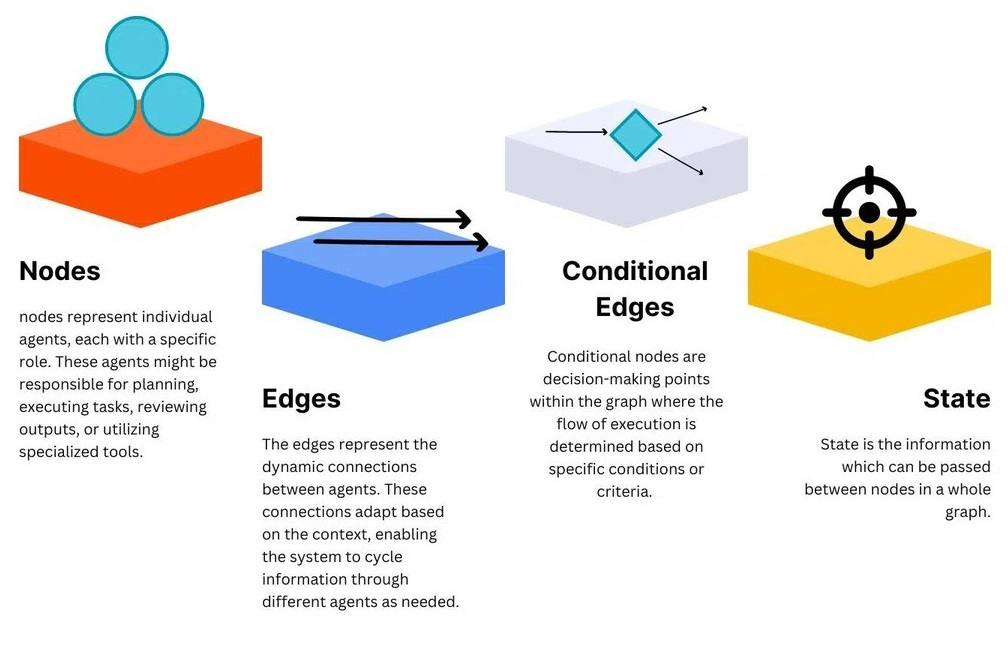
\includegraphics[scale = 0.5]{pictures/625723062_18126048418556935_1835132745978934341_n.jpg}
\caption{Các khái niệm quan trọng của LangGraph}
\end{figure}

Sơ đồ Agentic RAG dự án này:

\begin{figure}[H]
\centering
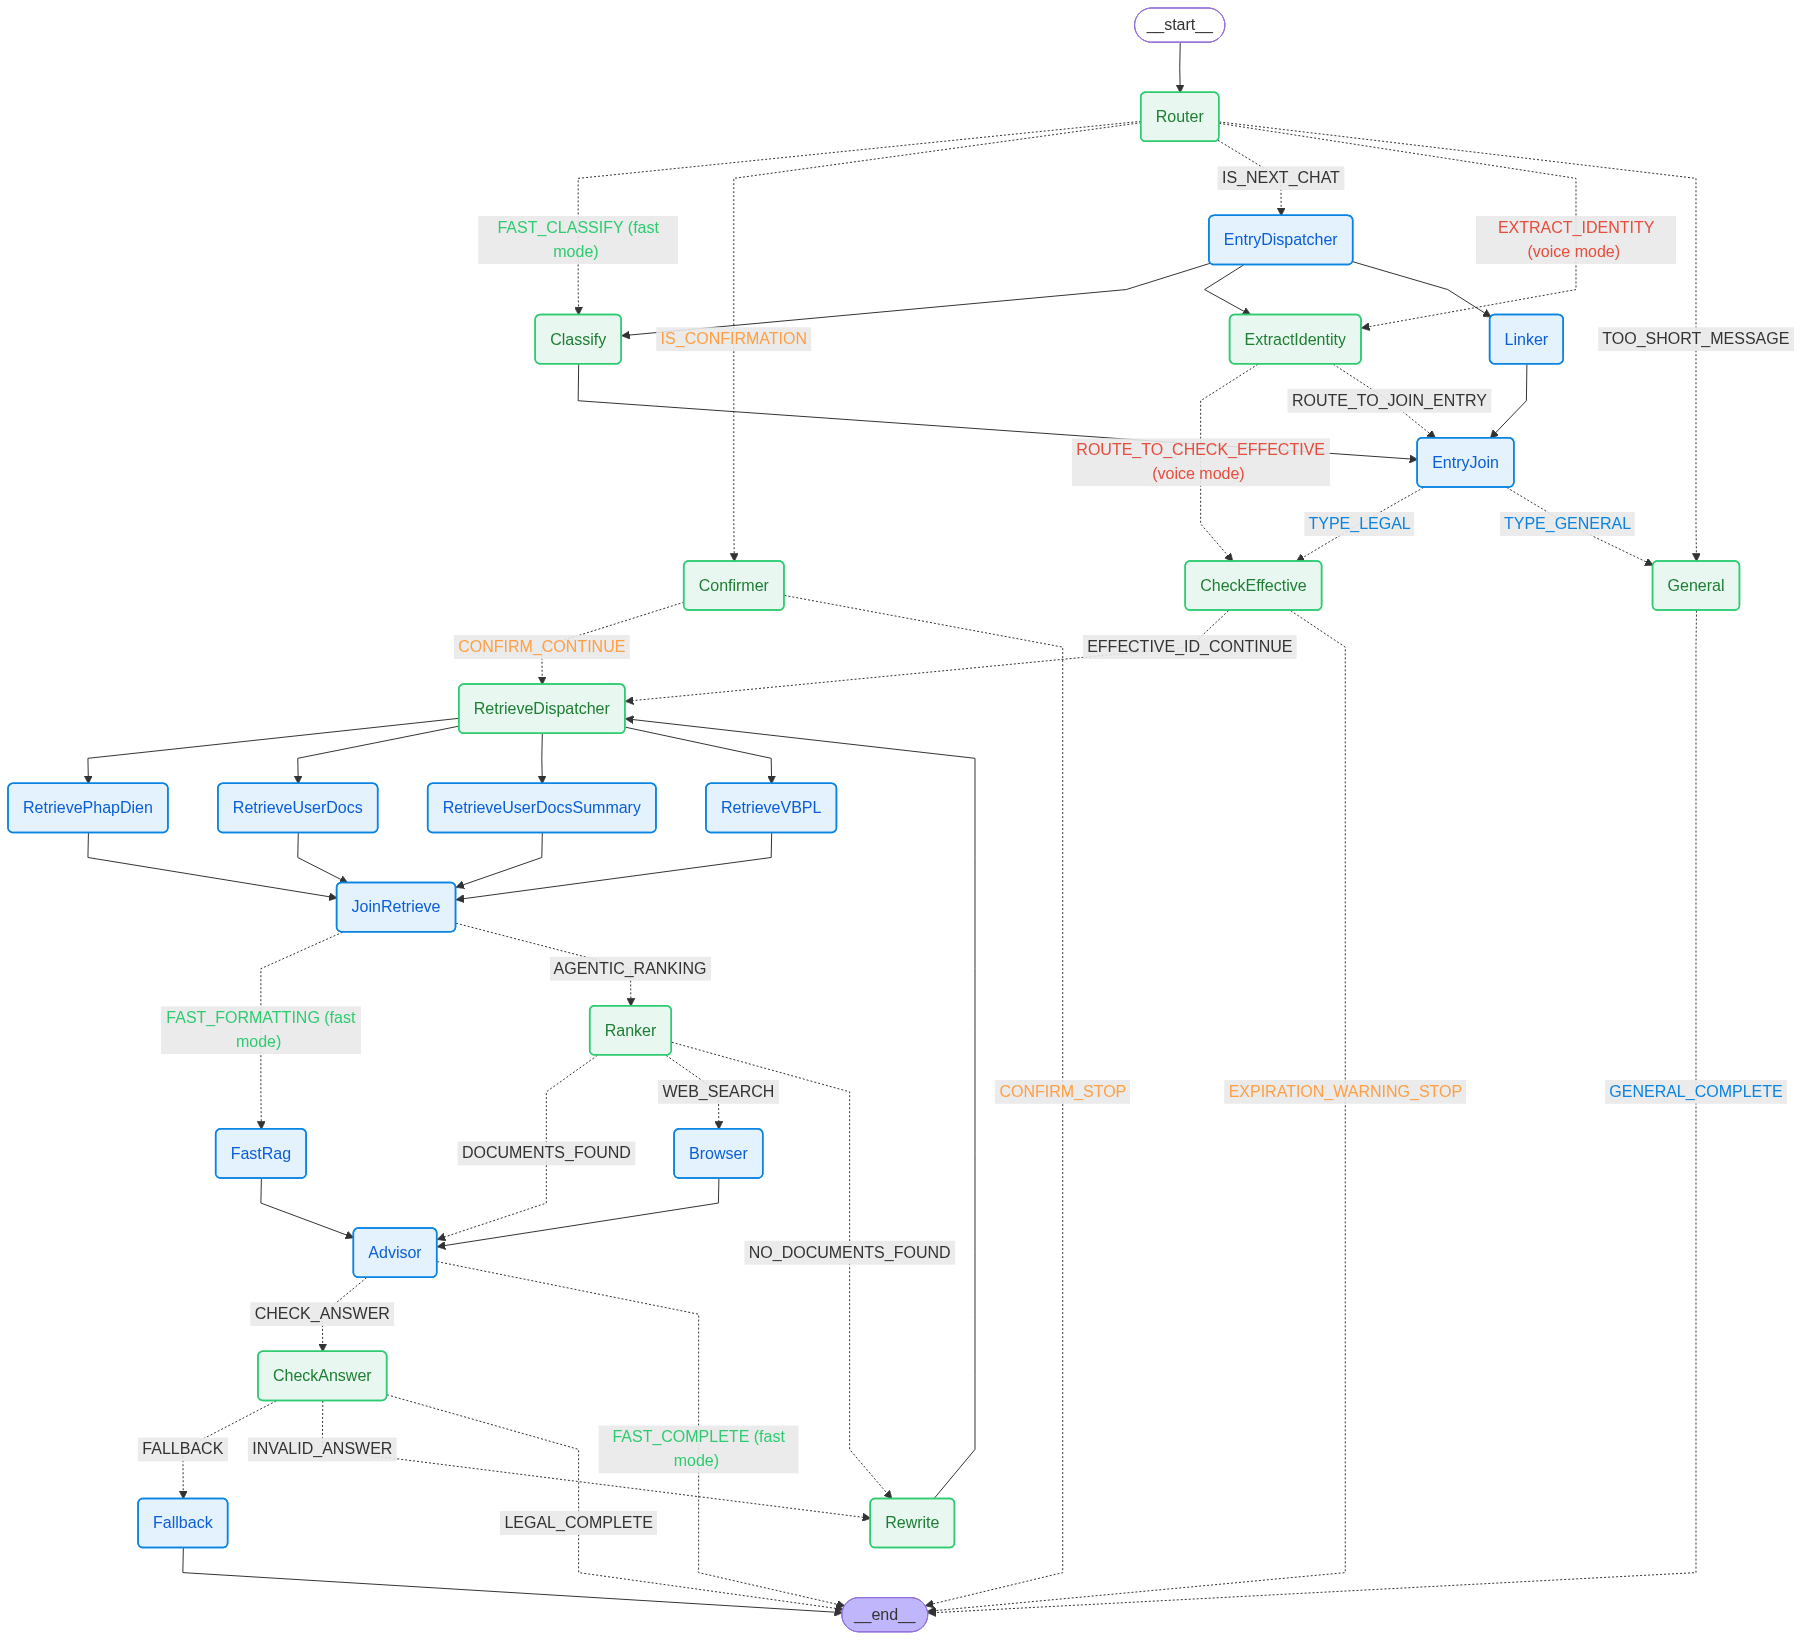
\includegraphics[scale = 0.23]{pictures/rag_diagram.png}
\caption{Sơ đồ LangGraph của dự án}
\end{figure}

Giải thích sơ đồ Agentic RAG:

\begin{itemize}
\item Hệ thống
phân chia việc sử dụng thông minh
giữa mô hình nhỏ cho luồng cơ bản
và mô hình lớn cho tác vụ suy luận
là chìa khóa để tối ưu cả chi phí, độ trễ và hiệu năng.
(Nhìn vào sơ đồ các Node màu xanh lá sử dụng mô hình nhỏ,
các Node màu xanh dương sử dụng mô hình lớn)

\item Mỗi tin nhắn đều đi qua \texttt{Router}.
Node này kiểm tra điều kiện
giúp định tuyến vào luồng chính xác
theo từng trạng thái.

\item Ở chế độ suy luận Agentic RAG đầy đủ
thực hiện
phân tích song song

\begin{itemize}

\item \texttt{Linker} đọc URL nếu có.
\item \texttt{Classify} phân loại câu hỏi là pháp lý hay thông thường.
\item \texttt{Extract Identity} trích xuất số hiệu văn bản (VD: \texttt{100/2019/NĐ-CP}).

\end{itemize}

\item Kiểm tra hiệu lực pháp lý:
Nếu câu hỏi thuộc nhóm \texttt{TYPE\_LEGAL} và có số hiệu văn bản,
hệ thống tra cứu trạng thái.

\begin{itemize}

\item Văn bản đã hết hiệu lực hoàn toàn
thì kết thúc ngay.
\item Văn bản hết hiệu lực một phần
thì phát cảnh báo và chờ người dùng xác nhận ở lượt sau qua \texttt{Confirmer}.

\end{itemize}

\item Truy xuất nguồn dữ liệu song song

\begin{itemize}

\item Tài liệu người dùng (Milvus)
\item Tóm tắt tài liệu (Cloudflare R2)
\item Văn bản pháp luật (Pinecone)
\item Dữ liệu pháp điển (Qdrant)

\end{itemize}

\item Tiếp tục tới \texttt{Ranker} để lọc tài liệu

\begin{itemize}

\item Nếu có tài liệu hợp lý
thì
chuyển đến \texttt{Advisor}
để tiến hành tạo câu trả lời.

\item Nếu không có tài liệu hợp lý
thì
chuyển đến \texttt{Rewrite}
để tạo lại câu hỏi.

\item Sau khi thử tạo lại câu hỏi
vẫn không có tài liệu hợp lý
thì sẽ dùng \texttt{Browser}
để lấy tài liệu
tại nguồn
thuvienphapluat.vn và luatvietnam.vn

\end{itemize}

\item Vòng lặp tự kiểm tra chất lượng
Sau khi \texttt{Advisor} trả lời,
\texttt{Check Answer} đánh giá câu trả lời có hợp lý hay không?

\begin{itemize}

\item Nếu không hợp lệ và chưa quá 2 lần
thì xóa câu trả lời cũ,
chuyển đến \texttt{Rewrite}
để tạo lại câu hỏi
và
lặp lại toàn bộ luồng truy xuất.

\item Nếu câu trả lời hợp lệ hoặc đã quá số lần thử lại
thì
hệ thống kết thúc quá trình trả lời.
\end{itemize}

\item Ở chế độ Fast RAG
chỉ đi qua \texttt{Classify} để phân loại.
Sau đó truy xuất dữ liệu lấy dữ liệu.
Dùng \texttt{Advisor} trả lời
và
hệ thống kết thúc quá trình trả lời
mà không cần bước kiểm tra.

\item Ở chế độ giọng nói Voice,
do đã có Agent nên không cần qua bước phân loại của LangGraph
và người dùng không thể nhập URL nên hệ thống chuyển đến \texttt{Extract Identity} trích xuất số hiệu văn bản.

\end{itemize}
 % Tuy nhiên, sử dụng RAG đơn giản
\input{contents/Kien_truc_vi_dich_vu_MSA_Microservice_Architecture} % Kiến trúc vi dịch vụ MSA (Microservice Architecture)
\input{contents/Thiet_ke_huong_mien_DDD_Domain_Driven_Design} % Thiết kế hướng miền DDD (Domain Driven Design)
\section{Phân tích thiết kế hệ thống}

\subsection{Bài toán nghiệp vụ}

Hệ thống hỗ trợ người dùng
hỏi đáp pháp luật Việt Nam,
phân tích tài liệu
và đàm thoại trực tiếp thời gian thực
với trợ lý ảo pháp lý.
Dựa trên thiết kế hướng miền (DDD),
bài toán lớn được chia làm
các miền phụ (Subdomain)
với các chức năng như sau:

\begin{figure}[H]
\centering
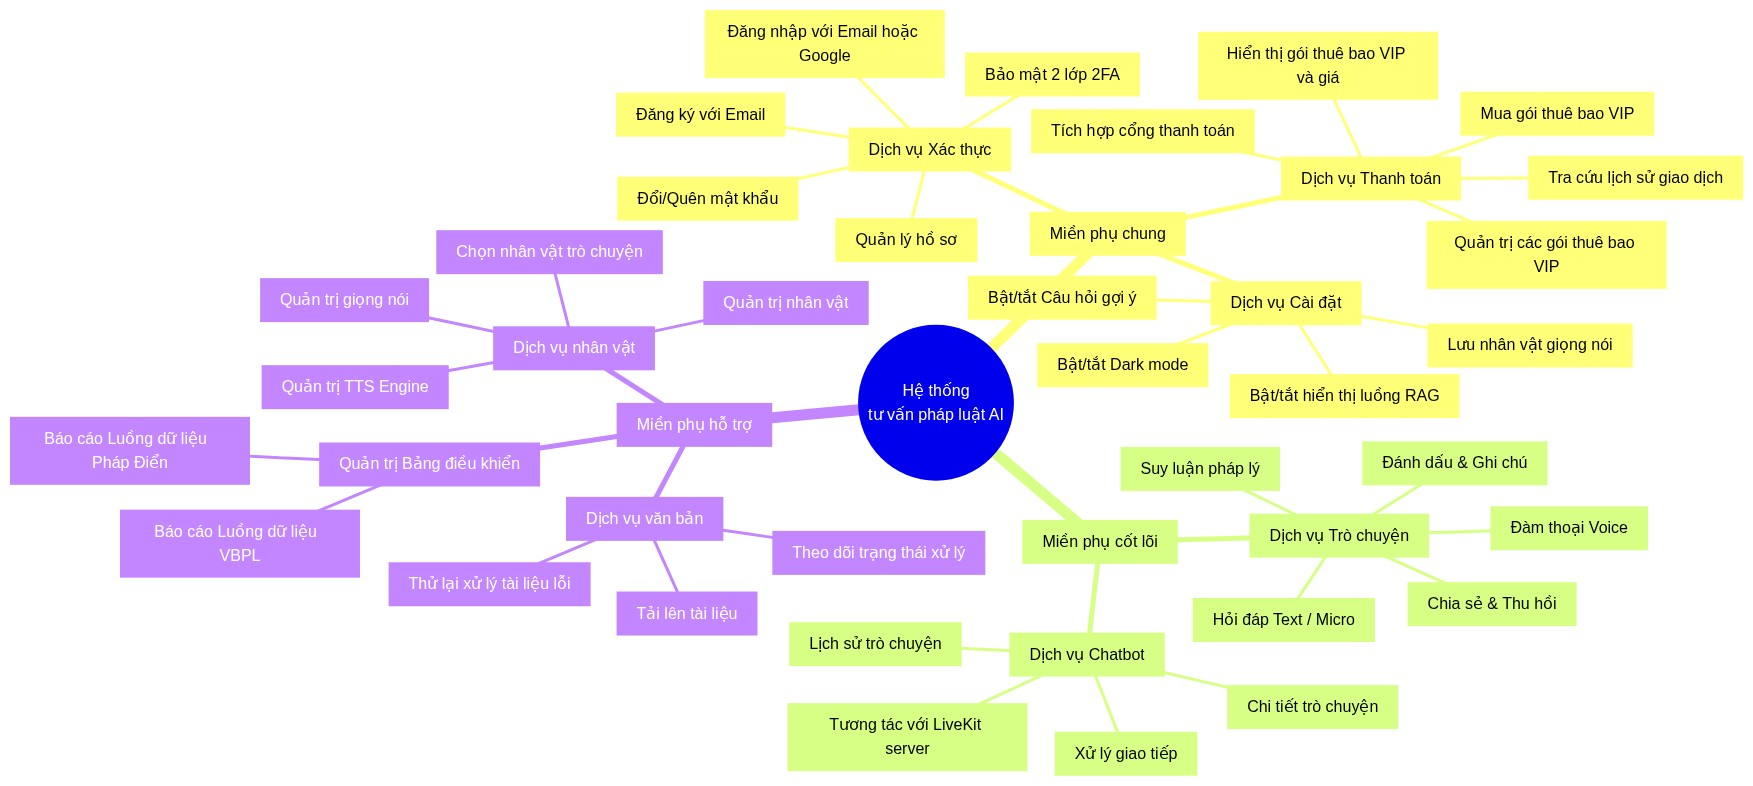
\includegraphics[scale = 0.25]{pictures/SubDomainMindMap.png}
\caption{Sơ đồ tổng quan SubDomain}
\end{figure}

\subsubsection{Miền phụ cốt lõi (Core Subdomain)}

Miền phụ cốt lõi
là phần quan trọng
và có giá trị nhất của hệ thống.
Miền phụ cốt lõi
giúp phân biệt các doanh nghiệp
và làm cho các doanh nghiệp có giá trị.
Miền phụ cốt lõi
tập trung vào mục tiêu
và yêu cầu của khách hàng với doanh nghiệp,
từ đó quyết định sự thành công của doanh nghiệp.
Vì vậy, mỗi doanh nghiệp
luôn tìm cách thực hiện những điều khác biệt
trong các miền phụ cốt lõi này để đạt được lợi thế so với đối thủ cạnh tranh.

% TODO: Subdomain-Core.tex
% TODO: Subdomain-Core.tex
% TODO: Subdomain-Core.tex

\input{contents/SubDomain-Core.tex} % \paragraph{Đặc điểm người dùng hệ thống}

Miền phụ cốt lõi
là nơi diễn ra các luồng xử lý phức tạp
và quyết định đến mức độ hài lòng của người dùng.

\subsubsection{Miền phụ hỗ trợ (Supporting Subdomain)}

Các miền phụ cốt lõi phụ thuộc
vào các miền phụ hỗ trợ.
Miền phụ hỗ trợ cung cấp các dịch vụ
để miền phụ cốt lõi hoạt động hiệu quả.
Tuy nhiên, miền phụ hỗ trợ không đòi hỏi mức độ phức tạp cao về logic nghiệp vụ.

% TODO: SubDomain-Supporting.tex
% TODO: SubDomain-Supporting.tex
% TODO: SubDomain-Supporting.tex

\input{contents/SubDomain-Supporting.tex} % \paragraph{Đặc điểm người dùng hệ thống}

Miền phụ hỗ trợ giúp miền phụ cốt lõi không bị phình to.
Tách nhỏ việc quản lý nhân vật, giọng nói
và quá trình xử lý tài liệu tiêu tốn nhiều tài nguyên hệ thống.

\subsubsection{Miền phụ chung (Generic Subdomain)}

Miền phụ chung
cung cấp các giải pháp có sẵn
mà doanh nghiệp có thể mua, thuê.
Miền phụ chung
có thể được tìm thấy trên nhiều ngành.
Doanh nghiệp không thể đạt được bất kỳ lợi thế cạnh tranh so
với đối thủ bằng cách thực hiện những điều khác biệt trong miền phụ chung.

% TODO: SubDomain-Generic.tex
% TODO: SubDomain-Generic.tex
% TODO: SubDomain-Generic.tex

\input{contents/SubDomain-Generic.tex} % \paragraph{Đặc điểm người dùng hệ thống}

Việc áp dụng các giải pháp có sẵn
như Supabase (Auth) hay Neon API (Settings)
là một chiến lược thông minh
để rút ngắn thời gian phát triển.
Đặc biệt là việc tích hợp 2FA,
điều kiện tiên quyết
cho các hệ thống xử lý hợp đồng
và dữ liệu pháp luật mang tính nhạy cảm.

Sơ đồ phân rã chức năng

\begin{figure}[H]
\centering
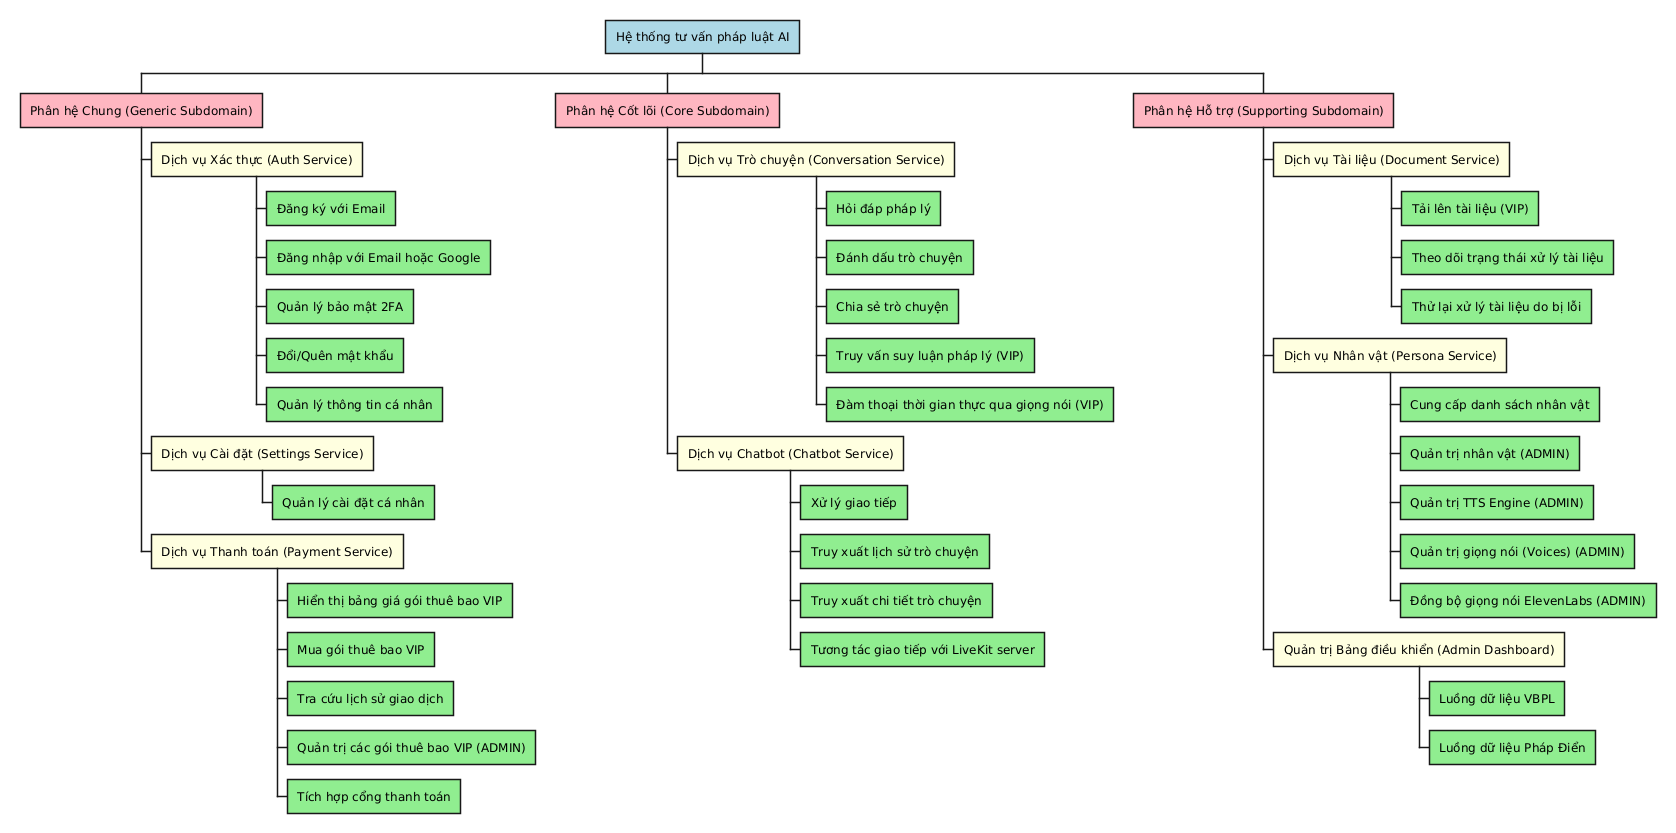
\includegraphics[scale = 0.18]{pictures/BFD.png}
\caption{Sơ đồ phân rã chức năng}
\end{figure}
 % Phân tích thiết kế hệ thống
\subsection{Giao diện chương trình}



% \newpage

{\centering \section*{KẾT LUẬN}}
\addcontentsline{toc}{section}{KẾT LUẬN}

LLM ( tinh chỉnh, ragas ....=> chọn model, cấu hình)

RAG
MICROSERVICE
Domain Driven Design
Data pipeline (air floww)
pay (xuất hóa đơn, event scing)

<!-- Stripe -->
tây nước ngoài có nhu cầu
<!-- payment trùng 2 lần -->

per (GPY Onivoi)
âm thanh giao diện sóng âm
<!-- Sóng âm (waveform animation) -->

chat thêm
<!-- feedback (0, 1) KHÓ vì microservice -->

test playwwringt

% \subsection*{Kết luận}

% Sau thời gian nghiên cứu, thiết kế và phát triển, đồ án tốt nghiệp với đề tài \textbf{“Xây dựng ứng dụng hỗ trợ tư vấn pháp luật sử dụng công nghệ trí tuệ nhân tạo”} đã hoàn thành đầy đủ các mục tiêu đề ra ban đầu, đáp ứng toàn bộ các yêu cầu kỹ thuật và nghiệp vụ được giao.

% Về kết quả đạt được, đồ án đã mang lại các giá trị cụ thể như sau:
% \begin{itemize}
% \item \textbf{Về mặt sản phẩm:} Xây dựng thành công một hệ thống trợ lý pháp luật hoàn chỉnh hoạt động dựa trên kiến trúc vi dịch vụ (Microservices) ổn định và dễ mở rộng. Trợ lý ảo AI sử dụng giải pháp Agentic RAG tiên tiến với LangGraph, cho phép trả lời các truy vấn pháp lý tiếng Việt một cách chính xác, minh bạch qua luồng suy luận rõ ràng và dẫn nguồn từ cơ sở dữ liệu pháp điển cũng như văn bản quy phạm pháp luật chính thống. Đồng thời, hệ thống hỗ trợ đàm thoại giọng nói thời gian thực và tự động hóa quy trình thanh toán thuê bao.
% \item \textbf{Về mặt công nghệ:} Làm chủ và tích hợp nhiều công nghệ hiện đại bao gồm NestJS, Python (LangGraph, FastAPI), gRPC, RabbitMQ, Apache Kafka, Qdrant Vector Database, cùng hạ tầng tự động hóa CI/CD, Docker và Kubernetes được quản lý qua GitOps (ArgoCD).
% \item \textbf{Về mặt kiến thức và kỹ năng tích lũy:} Qua quá trình thực hiện đồ án, sinh viên đã tích lũy được nhiều kiến thức chuyên sâu về xử lý ngôn ngữ tự nhiên (NLP), mô hình ngôn ngữ lớn (LLM), kiến trúc hệ thống phân tán và quy trình vận hành DevOps/GitOps. Đồng thời, sinh viên đã phát triển và nâng cao các kỹ năng quan trọng như: kỹ năng nghiên cứu khoa học, tự tìm kiếm và tổng hợp tài liệu chuyên ngành, kỹ năng lập kế hoạch và quản lý dự án, kỹ năng chế bản tài liệu chuyên nghiệp bằng LaTeX, cũng như kỹ năng viết báo cáo kỹ thuật.
% \end{itemize}

% Về mặt đánh giá, hệ thống cho thấy tính thực tiễn cao khi giải quyết được bài toán tra cứu thông tin pháp luật phức tạp. Tuy nhiên, tính chính xác của câu trả lời phụ thuộc nhiều vào chất lượng và độ cập nhật của cơ sở dữ liệu nguồn. Các mô hình AI vẫn đóng vai trò là một trợ lý hỗ trợ đắc lực và không thể thay thế hoàn toàn vai trò của các chuyên gia pháp lý trong các tình huống quyết định mang tính pháp lý cao.

% \subsection*{Hướng phát triển}

% Để hoàn thiện ứng dụng và nâng cao khả năng phục vụ người dùng trong thực tế, hướng phát triển của đồ án trong tương lai tập trung vào các nội dung sau:
% \begin{itemize}
% \item \textbf{Nâng cao chất lượng AI và tối ưu hóa RAG:} Nghiên cứu huấn luyện tinh chỉnh (Fine-tuning) mô hình nhúng (Embedding) trên tập dữ liệu luật Việt Nam; tích hợp mô hình Reranking để tăng độ chính xác khi tìm kiếm ngữ nghĩa; thử nghiệm các mô hình ngôn ngữ lớn chuyên biệt tiếng Việt mã nguồn mở nhằm nâng cao chất lượng câu trả lời và tự chủ dữ liệu.
% \item \textbf{Mở rộng tính năng nghiệp vụ:} Tích hợp công nghệ nhận dạng ký tự quang học (OCR) nâng cao để xử lý các tài liệu quét (scan PDF), hình ảnh pháp lý chất lượng kém từ phía người dùng; xây dựng hệ thống tự động theo dõi và gửi thông báo thay đổi hiệu lực của các văn bản pháp luật liên quan; mở rộng thêm các tính năng soạn thảo văn bản pháp lý tự động.
% \item \textbf{Tối ưu hiệu năng đàm thoại và hạ tầng:} Giảm thiểu tối đa độ trễ của các dịch vụ chuyển đổi giọng nói (STT và TTS) trong phân hệ Voice AI để nâng cao trải nghiệm đàm thoại thời gian thực; tối ưu hóa quy trình tự động co giãn (Auto-scaling) trên cụm Kubernetes nhằm đảm bảo tính sẵn sàng cao khi có lượng lớn người dùng truy cập đồng thời.
% \item \textbf{Đa dạng hóa nền tảng ứng dụng:} Phát triển các phiên bản ứng dụng di động (Mobile Application) trên hai hệ điều hành iOS và Android, giúp người dùng dễ dàng tiếp cận và sử dụng trợ lý pháp luật mọi lúc mọi nơi.
% \end{itemize}

\newpage

\newpage
{\centering \section*{TÀI LIỆU THAM KHẢO}}
\addcontentsline{toc}{section}{TÀI LIỆU THAM KHẢO}

\begingroup
\renewcommand{\section}[2]{} % Bỏ qua lệnh tạo tiêu đề tự động của thebibliography
\begin{thebibliography}{00}
\bibitem{nghia1} \url{https://vi.wikipedia.org/wiki/FPT}
\bibitem{nghia2} Tài liệu đào tạo hội nhập của Công ty TNHH FPT IS


% # https://neon.com/docs/data-api/custom-authentication-providers
% # <!-- # Tài liệu tham khảo -->
% # <!-- https://developer.hashicorp.com/terraform -->
% # <!-- https://github.com/features/actions -->
% # <!-- https://aws.amazon.com/vi/what-is/retrieval-augmented-generation -->
% # <!-- https://weaviate.io/blog/what-is-agentic-rag -->
% # <!-- https://dlthub.com/docs/intro -->
% # <!-- https://nestjs.com/ -->
% # <!-- https://fastapi.tiangolo.com/ -->
% # <!-- https://neon.com -->
% # <!-- https://supabase.com -->
% # <!-- https://www.scrapy.org -->
% # <!-- https://developer.konghq.com -->
% # https://grpc.io/ https://grpc.io/docs/

% # https://docs.livekit.io/reference/agents/events/
% # https://docs.livekit.io/reference/client-sdk-js/enums/RoomEvent.html
% # https://docs.livekit.io/intro/basics/rooms-participants-tracks/

\end{thebibliography}
\endgroup


% % \bibitem{nghia3} \url{https://fpt-is.com/san-pham-a-z}

% % \bibitem{nghia4} \url{https://fastapi.tiangolo.com}

% % \bibitem{nghia5} \url{https://docs.sqlalchemy.org/en/20}
% % \bibitem{nghia6} \url{https://alembic.sqlalchemy.org/en/latest/index.html}

% % \bibitem{nghia7} \url{https://www.rfc-editor.org/rfc/rfc7519}

% % \bibitem{nghia8} \url{https://pyjwt.readthedocs.io/en/stable}

% % \bibitem{nghia9} \url{https://pyauth.github.io/pyotp}

% % \bibitem{nghia10} \url{https://www.rfc-editor.org/rfc/rfc3174}
% % \bibitem{nghia11} \url{https://www.rfc-editor.org/rfc/rfc2104}
% % \bibitem{nghia12} \url{https://www.rfc-editor.org/rfc/rfc4226}
% % \bibitem{nghia13} \url{https://www.rfc-editor.org/rfc/rfc6238}

% % \bibitem{nghia14} \url{https://bind9.readthedocs.io/en/v9.20.4}

% % \bibitem{nghia15} \url{https://microservices.io}

% % \bibitem{nghia16} \url{https://docs.konghq.com/gateway/3.8.x}
% \end{thebibliography}

% \input{contents/0/trang_trang/trang_trang}

% % \url{https://example.com}




\begin{figure}[H]
    \centering
    
\includegraphics[scale = 0.2]{pictures/LogoHust.png}
    \caption{Logo của Đại học Bách Khoa Hà Nội}
\end{figure}

\begin{itemize}
    \item
          Nội dung mục 1
    \item
          Nội dung mục 2
    \item
        %   Nội dung mục 3
          Chấm màu xanh
\end{itemize}



% Chữ tạm màu đỏ
% Chữ demo màu đỏ 




\textit{In nghiêng đoạn văn bản}



\textbf{In đậm đoạn văn bản}



\begin{block}{Tiêu đề block}
    Nội dung block
\end{block}




% \textcolor{RedHUST}{\lipsum[1]}



Văn bản thông thường màu đen hiển thị ở đây.

\lipsum[1] % Đoạn này sẽ TỰ ĐỘNG có màu RedHUST

Văn bản bình thường tiếp theo không bị ảnh hưởng.

\lipsum[2-3] % Đoạn này cũng TỰ ĐỘNG có màu RedHUST



\lipsum[1]







\end{document}
